\makeatletter
\def\input@path{{../../}}
\makeatother
\documentclass[../../main.tex]{subfiles}

\graphicspath{
	{../../img/}
	{../img/}
	{img/}
}

\begin{document}
	
	\begin{thm}[Об интегральном предствалении производной ФКП]
        Если $f(z)$ аналитична в односвязной области $D$ 
        кусочно-гладкой границей и непрерывной в $D$, то 
        $f(z)$ бесконечно дифференцируема в $D$, причем 
        
        \begin{equation}
            \label{lec33:7}
            f^{(n)}(z_0) = \frac{n!}{2\pi i} \oint
            \frac{f(t)}{(t-z_0)^{n+1}} dz,
            t \in l, z \in D, n \in \N_0
        \end{equation}
        
	\end{thm}
	
	\begin{proof}
        Если $n=0$, то по интегральной формуле Коши
        \[
            f(z_0) = \frac{1}{2\pi i} \oint \limits_l
            \frac{f(t)}{t-z} dt, t \in l, z \in D
        \]
        Зафиксируем $t \in l$ и заключим $z \in D$ в
        некоторый компакт $D_0 \subset D$ с 
        кусочно-гладкой границей $l_0 = \partial D_0$
        положительно ориентированной. Тогда
        \[
         \begin{cases}
          \forall t \in l_0 \\
          \forall z \in D_0
         \end{cases} \implies t - z \neq 0
        \]
        Отсюда, в силу аналитичности $f(t)$ получаем, что
        \begin{equation}
         \label{lec33:9}
         \phi(t, z) = \frac{f(t)}{t-z} 
        \end{equation}
        аналитична как по $t$, так и по $z$, причем
        \[
            \exists\; \frac{\partial \phi(t, z)}{\partial z}
            = \frac{f(t)}{(t-z)^2}
            \text{ непрерывная на } b_0
        \]
        
        Тогда в силу теоремы о дифференцировании СИЗОП ФКП
        получаем, что 
        \begin{equation}
         \label{lec33:10}
         \exists f'(z) = \frac{1}{2\pi i} \oint\limits_{l_0}
         \frac{\partial \phi(t, z)}{\partial z} dt = 
         \frac{1}{2\pi i} \oint\limits_{l_0}\frac{f(t)}{(t-z)^2} 
         dt 
        \end{equation}
        
        Отсюда,учитывая замечание к интегральной формуле Коши 
        для много св. областей, имеем 
        \[
         f'(z) = \frac{1}{2\pi i} \oint \frac{f(t)}{(t-z)^2} dt
        \]
        то есть \eqref{lec33:7} задана для $n = 1$.
        Рассмотрим далее 
        \[
         \phi_1(t, z) = \frac{f(t)}{(t-z)^2}, t \in l_0,
         z \in D_0
        \]
        снова получим как и выше, что 
        \[
         \exists f''(z) = \frac{1}{2\pi i} \oint\limits_{l_0}
         \left( \frac{f(t)}{(t-z)^2} \right)' dt =
          \frac{2!}{2\pi i} \oint\limits_{l = \partial D}
          \frac{f(t)}{(t-z)^3} dt 
        \]
        и так далее обосновывается \eqref{lec33:7}
	\end{proof}
	\begin{rems}
	 \item[1.] Вывод \eqref{lec33:7} показывает, что $f(z)$ аналитична в 
	 $D$ бесконечное число раз дифференцируема в каждой точке
	 $D$.
	 \item[2.] \eqref{lec33:7} справедлива и для множеств
	  областей, но при этом под $l$ понимают полную границу $D$.
	  
	  \item[3.] Как и в случае интегральной формулы Коши, 
	  \eqref{lec33:7} можно переписать в виде 
	  \[
	   \oint\limits_l \frac{f(t)}{(t-z)^{n+1}} = 
	   \begin{cases}
	    \frac{2\pi i}{n!} f^{(n)}(z), z \in D \\
	    \text{иначе 0}
	   \end{cases}
	  \]
	  и исследовать её на практике для вычисления
	  соответствующего интеграла ФКП.
	\end{rems}
    \begin{exmp}
     \[
      I = \int\limits_{|z|=4}\frac{\cos z}{z^2 (z-\pi)}
      dz
     \]
     У подынтегральной функции $g(z)=\dfrac{\cos z}
     {z^2(z-\pi)}$ в круге $\abs{z} \leqslant 4$
     2 особые точки $z=0$ и $z=\pi$.
     
     \center{
     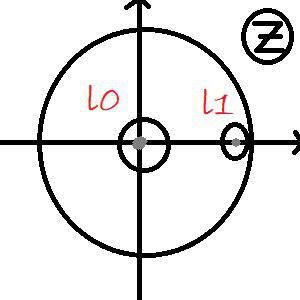
\includegraphics{lec33_1}}
     
     Отделяя особые точки и учитывая лемму об 
     интеграле от ФКП для многосвязной ФКП имеем 
     $I = I_0 + I_1$, где 
     \[
      I_0 = 
     \oint\limits_{l_0}\dfrac{\cos z}{z^2(z - \pi)} 
     dz=
     \oint\limits_{l_0}\dfrac{\frac{\cos z}
     {z-\pi}}{z^2} dz
     = \left[
     \begin{array}{l}
      f(z) = \dfrac{\cos z}{z-\pi} \\
     n = 1
     \end{array}
     \right] = 
     2\pi i \left( \dfrac{\cos z}{z-\pi}\right)'
     |_{z=0}=
     \]
     \[= -2\pi i \cdot \dfrac{\cos z + 
     (z - \pi) \sin z}{(z-\pi)^2}|_{z=0}=
     -2\pi i \cdot {1}{\pi ^2} = -\dfrac{2i}{\pi}
     \]

     \[
      I_1 = \oint_{l_1} \dfrac{\frac{\cos z}{z^2}}
      {z-\pi} dz = 2 \pi i \cdot \left(
      \dfrac{\cos z}{z^2}
      \right) |_{z=\pi} = 2\pi i \cdot \dfrac{-1}{\pi^2}
      =\dfrac{-2i}{\pi}.
     \]
     \[
      \implies I = I_0 + I_1 = -\dfrac{4i}{\pi}
     \]
    \end{exmp}

    \section{Некоторые приложения интегрального
    представления производных ФКП}
    
    Далее $f(z)$ дифференцируема $\forall z \in \C$
    будем называть целой ФКП.
    \begin{thm}[kek]
     Если целая $f(z)$ является ограниченной в $\C$,
     то есть
     \begin{equation}
     \label{lec33:11}
      \exists M = const > 0 : \abs{f(z)}
     \leqslant M, \forall z \in \C, 
     \end{equation}
     то тогда $f(z)$ тождественна равна константе.

    \end{thm}



\end{document}
